\documentclass{standalone}
\usepackage{tikz}
\usetikzlibrary{patterns, positioning}
\usetikzlibrary{shapes.misc}
\usepackage[outline]{contour}
\contourlength{1.5pt} 


\begin{document}
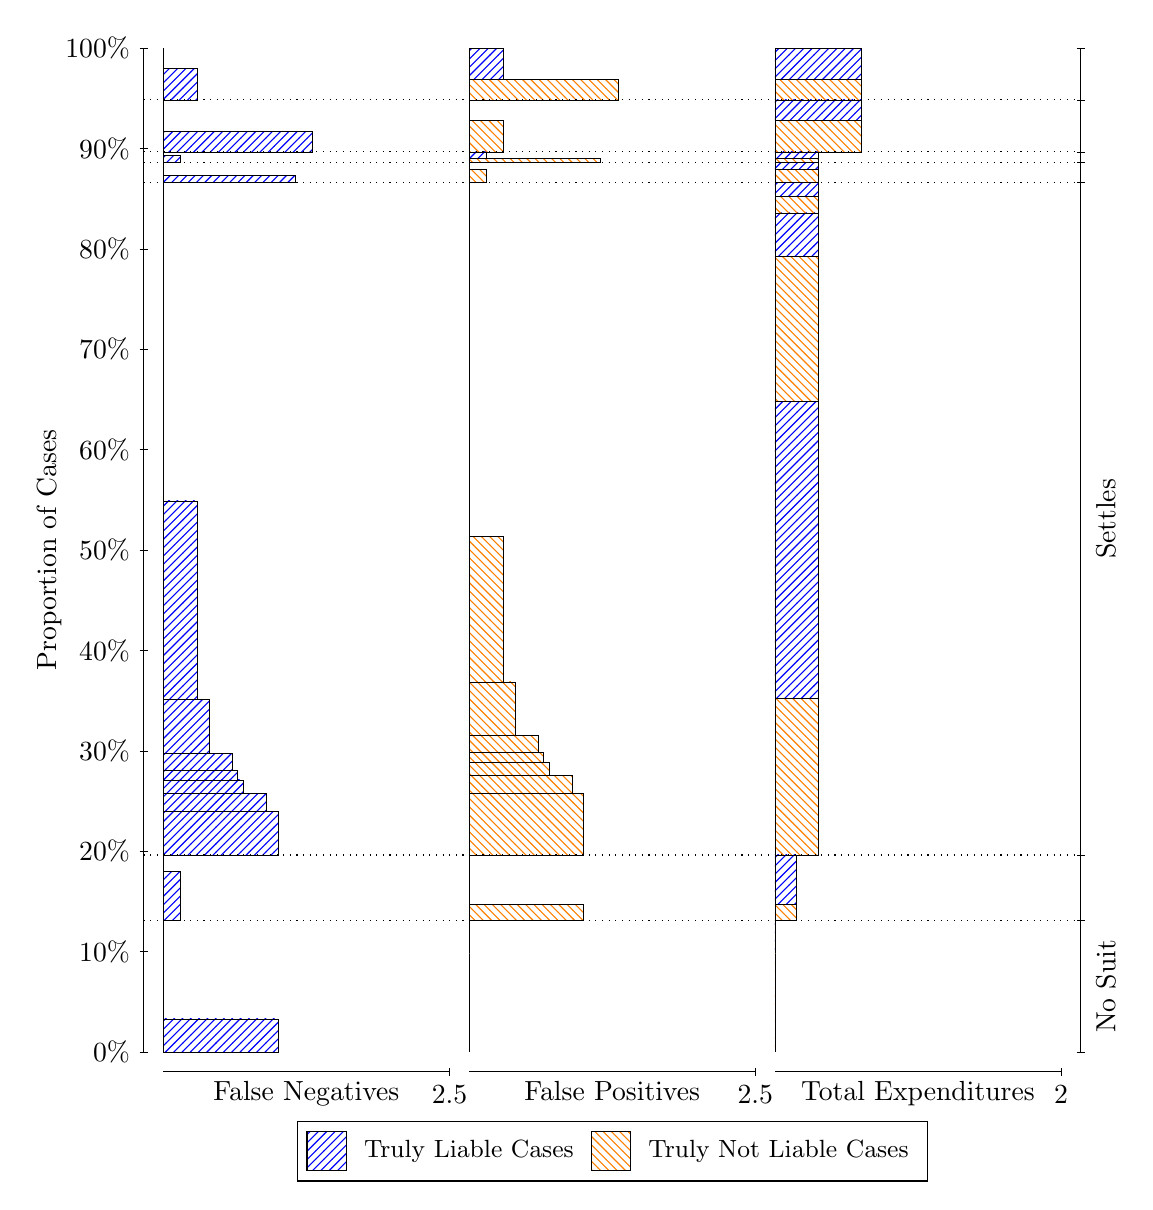
\begin{tikzpicture}
\draw[black, very thin] (1.5,1.75) -- (1.5,14.5);
\node[rotate=90, text=black, anchor=center] at (0.3, 8.125) {Proportion of Cases};
\draw[black, very thin] (1.45,1.75) -- (1.55,1.75);
\node[text=black, anchor=east] at (1.45, 1.75) {0\%};
\draw[black, very thin] (1.45,3.025) -- (1.55,3.025);
\node[text=black, anchor=east] at (1.45, 3.025) {10\%};
\draw[black, very thin] (1.45,4.3) -- (1.55,4.3);
\node[text=black, anchor=east] at (1.45, 4.3) {20\%};
\draw[black, very thin] (1.45,5.575) -- (1.55,5.575);
\node[text=black, anchor=east] at (1.45, 5.575) {30\%};
\draw[black, very thin] (1.45,6.85) -- (1.55,6.85);
\node[text=black, anchor=east] at (1.45, 6.85) {40\%};
\draw[black, very thin] (1.45,8.125) -- (1.55,8.125);
\node[text=black, anchor=east] at (1.45, 8.125) {50\%};
\draw[black, very thin] (1.45,9.4) -- (1.55,9.4);
\node[text=black, anchor=east] at (1.45, 9.4) {60\%};
\draw[black, very thin] (1.45,10.675) -- (1.55,10.675);
\node[text=black, anchor=east] at (1.45, 10.675) {70\%};
\draw[black, very thin] (1.45,11.95) -- (1.55,11.95);
\node[text=black, anchor=east] at (1.45, 11.95) {80\%};
\draw[black, very thin] (1.45,13.225) -- (1.55,13.225);
\node[text=black, anchor=east] at (1.45, 13.225) {90\%};
\draw[black, very thin] (1.45,14.5) -- (1.55,14.5);
\node[text=black, anchor=east] at (1.45, 14.5) {100\%};

\draw[black, very thin] (13.4,1.75) -- (13.4,14.5);
\draw[black, very thin] (13.35,1.75) -- (13.45,1.75);
\node[anchor=west] at (13.35, 1.75) {};
\draw[black, very thin] (13.35,3.4177) -- (13.45,3.4177);
\node[anchor=west] at (13.35, 3.4177) {};
\draw[black, very thin] (13.35,4.2516) -- (13.45,4.2516);
\node[anchor=west] at (13.35, 4.2516) {};
\draw[black, very thin] (13.35,12.79) -- (13.45,12.79);
\node[anchor=west] at (13.35, 12.79) {};
\draw[black, very thin] (13.35,13.051) -- (13.45,13.051);
\node[anchor=west] at (13.35, 13.051) {};
\draw[black, very thin] (13.35,13.182) -- (13.45,13.182);
\node[anchor=west] at (13.35, 13.182) {};
\draw[black, very thin] (13.35,13.841) -- (13.45,13.841);
\node[anchor=west] at (13.35, 13.841) {};
\draw[black, very thin] (13.35,14.5) -- (13.45,14.5);
\node[anchor=west] at (13.35, 14.5) {};

\draw[black, very thin, pattern color=blue, pattern=north east lines] (1.75,1.75) rectangle (3.2033,2.1699);
\draw[black, very thin, pattern color=orange, pattern=north west lines] (1.75,2.1699) rectangle (1.75,3.4177);
\draw[black, very thin, pattern color=blue, pattern=north east lines] (1.75,3.4177) rectangle (1.968,4.0416);
\draw[black, very thin, pattern color=orange, pattern=north west lines] (1.75,4.0416) rectangle (1.75,4.2516);
\draw[black, very thin, pattern color=blue, pattern=north east lines] (1.75,4.2516) rectangle (3.2033,4.8058);
\draw[black, very thin, pattern color=blue, pattern=north east lines] (1.75,4.8058) rectangle (3.058,5.033);
\draw[black, very thin, pattern color=blue, pattern=north east lines] (1.75,5.033) rectangle (2.7673,5.2045);
\draw[black, very thin, pattern color=blue, pattern=north east lines] (1.75,5.2045) rectangle (2.6947,5.3307);
\draw[black, very thin, pattern color=blue, pattern=north east lines] (1.75,5.3307) rectangle (2.622,5.5422);
\draw[black, very thin, pattern color=blue, pattern=north east lines] (1.75,5.5422) rectangle (2.3313,6.2231);
\draw[black, very thin, pattern color=blue, pattern=north east lines] (1.75,6.2231) rectangle (2.186,8.7475);
\draw[black, very thin, pattern color=orange, pattern=north west lines] (1.75,8.7475) rectangle (1.75,12.79);
\draw[black, very thin, pattern color=blue, pattern=north east lines] (1.75,12.79) rectangle (3.4213,12.881);
\draw[black, very thin, pattern color=orange, pattern=north west lines] (1.75,12.881) rectangle (1.75,13.051);
\draw[black, very thin, pattern color=blue, pattern=north east lines] (1.75,13.051) rectangle (1.968,13.137);
\draw[black, very thin, pattern color=orange, pattern=north west lines] (1.75,13.137) rectangle (1.75,13.182);
\draw[black, very thin, pattern color=blue, pattern=north east lines] (1.75,13.182) rectangle (3.6393,13.445);
\draw[black, very thin, pattern color=orange, pattern=north west lines] (1.75,13.445) rectangle (1.75,13.841);
\draw[black, very thin, pattern color=blue, pattern=north east lines] (1.75,13.841) rectangle (2.186,14.237);
\draw[black, very thin, pattern color=orange, pattern=north west lines] (1.75,14.237) rectangle (1.75,14.5);
\draw[black, very thin, pattern color=orange, pattern=north west lines] (5.6333,1.75) rectangle (5.6333,2.9978);
\draw[black, very thin, pattern color=blue, pattern=north east lines] (5.6333,2.9978) rectangle (5.6333,3.4177);
\draw[black, very thin, pattern color=orange, pattern=north west lines] (5.6333,3.4177) rectangle (7.0867,3.6277);
\draw[black, very thin, pattern color=blue, pattern=north east lines] (5.6333,3.6277) rectangle (5.6333,4.2516);
\draw[black, very thin, pattern color=orange, pattern=north west lines] (5.6333,4.2516) rectangle (7.0867,5.0329);
\draw[black, very thin, pattern color=orange, pattern=north west lines] (5.6333,5.0329) rectangle (6.9413,5.2601);
\draw[black, very thin, pattern color=orange, pattern=north west lines] (5.6333,5.2601) rectangle (6.6507,5.4316);
\draw[black, very thin, pattern color=orange, pattern=north west lines] (5.6333,5.4316) rectangle (6.578,5.5578);
\draw[black, very thin, pattern color=orange, pattern=north west lines] (5.6333,5.5578) rectangle (6.5053,5.7693);
\draw[black, very thin, pattern color=orange, pattern=north west lines] (5.6333,5.7693) rectangle (6.2147,6.4503);
\draw[black, very thin, pattern color=orange, pattern=north west lines] (5.6333,6.4503) rectangle (6.0693,8.2938);
\draw[black, very thin, pattern color=blue, pattern=north east lines] (5.6333,8.2938) rectangle (5.6333,12.79);
\draw[black, very thin, pattern color=orange, pattern=north west lines] (5.6333,12.79) rectangle (5.8513,12.96);
\draw[black, very thin, pattern color=blue, pattern=north east lines] (5.6333,12.96) rectangle (5.6333,13.051);
\draw[black, very thin, pattern color=orange, pattern=north west lines] (5.6333,13.051) rectangle (7.3047,13.097);
\draw[black, very thin, pattern color=blue, pattern=north east lines] (5.6333,13.097) rectangle (5.8513,13.182);
\draw[black, very thin, pattern color=orange, pattern=north west lines] (5.6333,13.182) rectangle (6.0693,13.578);
\draw[black, very thin, pattern color=blue, pattern=north east lines] (5.6333,13.578) rectangle (5.6333,13.841);
\draw[black, very thin, pattern color=orange, pattern=north west lines] (5.6333,13.841) rectangle (7.5227,14.104);
\draw[black, very thin, pattern color=blue, pattern=north east lines] (5.6333,14.104) rectangle (6.0693,14.5);
\draw[black, very thin, pattern color=orange, pattern=north west lines] (9.5167,1.75) rectangle (9.5167,2.9978);
\draw[black, very thin, pattern color=blue, pattern=north east lines] (9.5167,2.9978) rectangle (9.5167,3.4177);
\draw[black, very thin, pattern color=orange, pattern=north west lines] (9.5167,3.4177) rectangle (9.7892,3.6277);
\draw[black, very thin, pattern color=blue, pattern=north east lines] (9.5167,3.6277) rectangle (9.7892,4.2516);
\draw[black, very thin, pattern color=orange, pattern=north west lines] (9.5167,4.2516) rectangle (10.062,6.2388);
\draw[black, very thin, pattern color=blue, pattern=north east lines] (9.5167,6.2388) rectangle (10.062,10.009);
\draw[black, very thin, pattern color=orange, pattern=north west lines] (9.5167,10.009) rectangle (10.062,11.852);
\draw[black, very thin, pattern color=blue, pattern=north east lines] (9.5167,11.852) rectangle (10.062,12.407);
\draw[black, very thin, pattern color=orange, pattern=north west lines] (9.5167,12.407) rectangle (10.062,12.618);
\draw[black, very thin, pattern color=blue, pattern=north east lines] (9.5167,12.618) rectangle (10.062,12.79);
\draw[black, very thin, pattern color=orange, pattern=north west lines] (9.5167,12.79) rectangle (10.062,12.96);
\draw[black, very thin, pattern color=blue, pattern=north east lines] (9.5167,12.96) rectangle (10.062,13.051);
\draw[black, very thin, pattern color=orange, pattern=north west lines] (9.5167,13.051) rectangle (10.062,13.097);
\draw[black, very thin, pattern color=blue, pattern=north east lines] (9.5167,13.097) rectangle (10.062,13.182);
\draw[black, very thin, pattern color=orange, pattern=north west lines] (9.5167,13.182) rectangle (10.607,13.578);
\draw[black, very thin, pattern color=blue, pattern=north east lines] (9.5167,13.578) rectangle (10.607,13.841);
\draw[black, very thin, pattern color=orange, pattern=north west lines] (9.5167,13.841) rectangle (10.607,14.104);
\draw[black, very thin, pattern color=blue, pattern=north east lines] (9.5167,14.104) rectangle (10.607,14.5);
\draw[black, dotted] (1.5,3.4177) -- (13.4,3.4177);
\draw[black, dotted] (1.5,4.2516) -- (13.4,4.2516);
\draw[black, dotted] (1.5,12.79) -- (13.4,12.79);
\draw[black, dotted] (1.5,13.051) -- (13.4,13.051);
\draw[black, dotted] (1.5,13.182) -- (13.4,13.182);
\draw[black, dotted] (1.5,13.841) -- (13.4,13.841);
\draw[black, very thin] (1.75,1.5) -- (5.3833,1.5);
\node[text=black, anchor=north] at (3.5667, 1.5) {False Negatives};
\draw[black, very thin] (5.3833,1.45) -- (5.3833,1.55);
\node[text=black, anchor=north] at (5.3833, 1.45) {2.5};

\draw[black, very thin] (5.6333,1.5) -- (9.2667,1.5);
\node[text=black, anchor=north] at (7.45, 1.5) {False Positives};
\draw[black, very thin] (9.2667,1.45) -- (9.2667,1.55);
\node[text=black, anchor=north] at (9.2667, 1.45) {2.5};

\draw[black, very thin] (9.5167,1.5) -- (13.15,1.5);
\node[text=black, anchor=north] at (11.333, 1.5) {Total Expenditures};
\draw[black, very thin] (13.15,1.45) -- (13.15,1.55);
\node[text=black, anchor=north] at (13.15, 1.45) {2};

\node[text=black, centered, rotate=90] at (13.72, 2.5839) {\contour{white}{No Suit}};

\node[text=black, centered, rotate=90] at (13.72, 8.5207) {\contour{white}{Settles}};





\draw (7.449999999999999,1.5) node[draw=none] (baseCoordinate) {};
\begin{scope}[align=center]
        \matrix[scale=0.5, draw=black, below=0.5cm of baseCoordinate, nodes={draw}, column sep=0.1cm]{
            \node[rectangle, draw, minimum width=0.5cm, minimum height=0.5cm, pattern color=blue, pattern=north east lines] {}; &
            \node[draw=none, font=\small, text=black] (B) {Truly Liable Cases}; &
            \node[rectangle, draw, minimum width=0.5cm, minimum height=0.5cm, pattern color=orange, pattern=north west lines] {}; &
            \node[draw=none, font=\small, text=black] (B) {Truly Not Liable Cases}; \\
            };
\end{scope}

\end{tikzpicture}
\end{document}